% Appendix: Point-process background and estimation reference.
% Pedagogical companion to Sections 2--5 of the main paper.

\section{Point-process background --- every term defined}
\label{app:pp-background}

This appendix builds the vocabulary from scratch. If you already know what a $\sigma$-algebra is you can skim to \S\ref{app:pp-intensity}, but the paper is meant to be readable by people who don't.

\subsection*{Warm-up: the Poisson process in plain English}
\label{app:pp-warmup}

Before defining a ``point process'' formally, meet its simplest member: the Poisson process. Once you're comfortable with this, the rest of the appendix is just formalising it and generalising it.

\paragraph{The setup.} Imagine you're watching messages arrive from a market-data feed and you write down the time of each arrival:

\begin{verbatim}
09:30:00.213    <- 1st arrival
09:30:00.451    <- 2nd
09:30:00.802    <- 3rd
09:30:01.014    <- 4th
09:30:01.317    <- 5th
...
\end{verbatim}

That list of timestamps is the raw thing we're going to model. Nothing else --- no prices, no sides, just when.

\paragraph{The Poisson idea.} Imagine that every very-tiny fraction of a second, there is some \emph{small independent} chance an arrival happens. Independent means: whether one arrives right now doesn't depend on when the previous one came, or how many happened in the last minute, or anything about the past. It's like flipping a huge number of very-biased coins, one for each tiny sliver of time, and calling an arrival every time one comes up heads.

The \emph{rate} of the process is a single number, usually written $\lambda$ (``lambda'', for now think ``rate'') or $\mu$ (``mu''), in units of \emph{arrivals per second}. Concretely, if the rate is 300 per second:
$$\mu = 300\ \text{arrivals per second},$$
then on average you get 300 arrivals per second, forever.

Three consequences that follow purely from ``each tiny sliver is independent'':

\paragraph{(1) The time between consecutive arrivals (``gap'') follows an exponential distribution with mean $1/\mu$.} If $\mu = 300$ per second, the mean gap is
$$\text{mean gap} = \frac{1}{\mu} = \frac{1}{300/\mathrm{s}} \approx 3.3\ \mathrm{ms}.$$
The gap distribution has the memoryless property: no matter how long you've been waiting, the expected time to the next arrival is still 3.3\,ms. The probability the next gap exceeds some time $\Delta$ is
$$\Pr(\text{gap} > \Delta) = e^{-\mu\,\Delta}.$$
Substituting our example rate gives $\Pr(\text{gap} > 3.3\,\mathrm{ms}) \approx 36.8\%$, $\Pr(\text{gap} > 6.6\,\mathrm{ms}) \approx 13.5\%$, $\Pr(\text{gap} > 10\,\mathrm{ms}) \approx 5.0\%$. Conversely, the probability the gap is shorter than one-tenth of the mean is
$$\Pr\!\big(\text{gap} < \tfrac{1}{10}\,\text{mean}\big) = 1 - e^{-0.1} \approx 9.52\%.$$
This $9.52\%$ number appears again in the rest of the paper. It's the Poisson benchmark for ``how often do two arrivals come nearly back-to-back''. If empirical data shows 60--85\% instead of 9.52\%, we've rejected Poisson.

\begin{figure}[H]
    \centering
    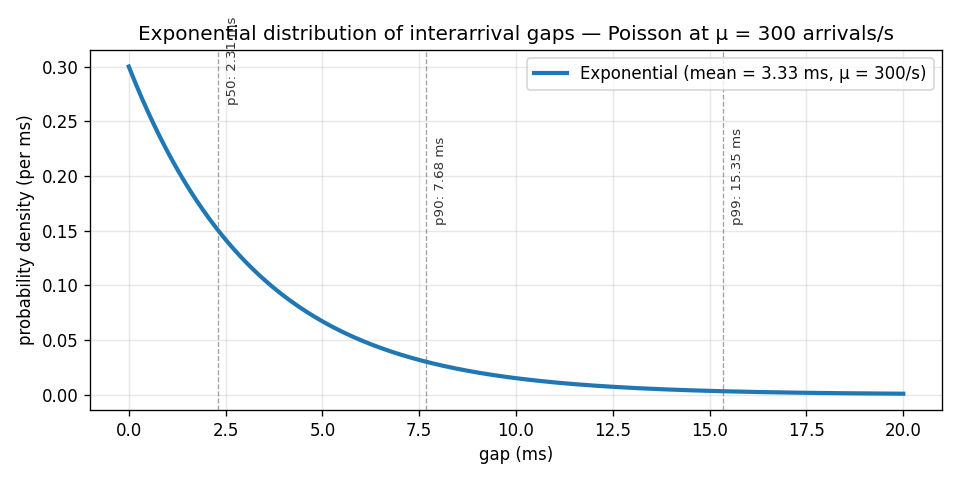
\includegraphics[width=0.75\textwidth]{figs/exponential_gaps.png}
    \caption{The exponential PDF of interarrival gaps for a rate-$300/$s Poisson process. Dashed vertical lines mark the p50 (median), p90, and p99 quantiles. Under Poisson, half the gaps are shorter than the median 2.3\,ms and 10\% are longer than 7.7\,ms --- a specific shape with a soft right tail. Real CME MDP3 data has a completely different shape: far more mass near 0 (bunched arrivals) and a much heavier right tail (long quiet stretches).}
    \label{fig:exponential-gaps}
\end{figure}

\paragraph{(2) The count in any window of length $T$ is Poisson-distributed.} Let $C$ be the count of arrivals in a window of length $T$:
$$\mathrm{E}[C] = \mu T, \qquad \mathrm{Var}[C] = \mu T$$
(same as the mean --- that's the defining property of a Poisson distribution). So the ratio of variance to mean in \emph{any} window $T$ is
$$\frac{\mathrm{Var}[C]}{\mathrm{E}[C]} = 1$$
always. This ratio is called the \textbf{Fano factor} (\S\ref{app:pp-fano} formally defines this); Poisson gives Fano $= 1$ at every window size. Any departure from this is a rejection of Poisson.

\paragraph{(3) The count in disjoint windows is independent.} Whatever happened in $[0, 1\,\mathrm{s}]$ tells you nothing about how many arrivals happen in $[1\,\mathrm{s}, 2\,\mathrm{s}]$. No memory, no clustering, no repulsion --- just independence.

\paragraph{Why Poisson is the ``null hypothesis'' everyone starts from.} Poisson is what happens if arrivals are ``as random as possible'' --- no self-reinforcement, no clustering, no bunching, no memory. It's what a purely mechanical, uncoordinated source would look like. Every departure from Poisson tells us something about the market: bursts of information, coordinated flow, self-reinforcing feedback.

\paragraph{Two ways real market data rejects Poisson.} \emph{Bunching}: real messages arrive in bursts. Many gaps are far shorter than the exponential mean would predict --- in ES/NQ we see 60--85\% of gaps shorter than mean$/10$, versus Poisson's 9.52\%. \emph{Momentum in the intensity}: after a burst starts, more arrivals are likely to keep coming. That's the opposite of Poisson's memoryless assumption. To model these, we need a class of processes that is Poisson-like locally (arrivals still happen randomly on tiny timescales) but where the \emph{rate} itself changes with the history. That's exactly a \textbf{conditional-intensity point process}.

\paragraph{Notational note.} Some authors write the Poisson rate as $\lambda$, others as $\mu$. In this appendix $\mu$ is reserved for the \emph{background} rate of a Hawkes process (which reduces to plain Poisson when the excitation kernel is zero), and $\lambda(t)$ is reserved for the general time-varying conditional intensity. For a plain Poisson process, $\lambda(t) = \mu$ for all $t$.

\subsection{What is a point process and what is a point}
\label{app:pp-pointprocess}

\begin{itemize}
    \item A \textbf{point} here means a single instant in time when something happens. Not a spatial point, not a decimal point. Just one instant --- the timestamp of one message arriving from the CME feed.
    \item A \textbf{process} is a random object that unfolds in time. A coin flipped once is random but static; a stock price ticking through the day is a random \emph{process}. In our case the process produces a random \emph{list of arrival timestamps} $t_1, t_2, t_3, \ldots$
    \item A \textbf{point process} is a random sequence of points (timestamps) on the real line, specified by \emph{when} events happen and nothing else.
\end{itemize}

If each event also carries additional information (side, price, size), that's a \textbf{marked point process} --- the timestamps are the ``points'' and the additional info per event is called a \textbf{mark}. Our arrival streams are naturally marked, but for arrival-process characterisation we mostly ignore the marks and treat only the timestamps as the process.

Alternative names in the literature: ``counting process'' (emphasises $N(t)$), ``temporal point process'' (distinguishes from spatial), ``renewal process'' (a specific subclass --- \S\ref{app:pp-canon}b), ``self-exciting process'' (Hawkes --- \S\ref{app:pp-canon}c).

\paragraph{Concrete example.} Between 09:30:00 and 09:30:01 of NQ March 2025 the following four MBO arrivals occur:
\begin{verbatim}
09:30:00.001234567   Add,    bid 21432.50, size 3
09:30:00.001234571   Add,    ask 21432.75, size 5
09:30:00.017891234   Cancel, order X, bid 21432.25
09:30:00.238491702   Trade,  ask 21432.75, size 2
\end{verbatim}
The point process is just the four timestamps. The marks (Add/Cancel/Trade, side, price, size) are additional per-event data.

\subsection{The setup: a probability space}
\label{app:pp-probspace}

We model market-data arrivals as a \textbf{stochastic process}: a family of random variables indexed by time. The underlying machinery is a probability space $(\Omega, \mathcal{F}, \Pr)$:

\begin{itemize}
    \item $\Omega$ (``sample space'') --- the set of all possible outcomes of the whole experiment. Here an outcome is one specific realisation of the market's day: the complete list of arrival timestamps, prices, sides, etc. You never see $\Omega$ directly; it exists to make everything else well-defined.
    \item $\mathcal{F}$ (``$\sigma$-algebra'') --- think of it as the exhaustive list of yes-or-no questions we're allowed to ask about the outcome and to which a probability can be assigned. Each such question corresponds to a subset of $\Omega$: the subset for which the answer is ``yes''. Two examples: ``did at least one message arrive between 09:30:00 and 09:30:01?'' and ``did the front contract trade above 21500 at some point?'' The two rules a $\sigma$-algebra must satisfy just say the catalog is closed under negation and countable union. Every event you'd naturally think of lives in it. For our timestamp setting, $\mathcal{F}$ is the standard Borel $\sigma$-algebra --- the natural catalog of yes/no questions on the real line.
    \item $\Pr : \mathcal{F} \to [0, 1]$ --- assigns a probability to each event. Satisfies $\Pr(\emptyset) = 0$, $\Pr(\Omega) = 1$, and countable additivity on disjoint events.
\end{itemize}

\subsection{Filtration: how information accumulates over time}
\label{app:pp-filtration}

At time $t = 0$ we know nothing yet. As time passes we observe more arrivals. To formalise this we use a \textbf{filtration}, an increasing family of $\sigma$-algebras:
$$\{\mathcal{F}_t\}_{t \geq 0}, \qquad \mathcal{F}_s \subset \mathcal{F}_t \text{ for } s \leq t.$$
$\mathcal{F}_t$ is the $\sigma$-algebra of everything observable by time $t$ inclusive. $\mathcal{F}_{t^-}$ is everything observable strictly before $t$. When a formula says ``conditional on $\mathcal{F}_{t^-}$'', it means ``given everything we've seen strictly before time $t$''. A process is \emph{adapted} to $\{\mathcal{F}_t\}$ if for every $t$ its value is measurable with respect to $\mathcal{F}_t$ --- i.e., knowable from the history up to $t$.

\subsection{The counting process $N(t)$}
\label{app:pp-counting}

The observable object is a random function of time:
$$N(t) = \#\{\, i : t_i \leq t \,\}.$$
$t_1, t_2, \ldots$ are the (random) arrival times; $N(t)$ is a non-decreasing, right-continuous, step function of $t$ that jumps by 1 at each arrival with $N(0) = 0$. The number of arrivals in a half-open interval is
$$N(t + h) - N(t) = \text{number of arrivals in }(t, t + h].$$

\subsection{Conditional intensity: the current speed of the process}
\label{app:pp-intensity}

\paragraph{Plain English first.} At any moment $t$, ask two questions: (1) ``what's the probability that at least one new message arrives in the next tiny sliver of time, of length $h$ seconds?'' and (2) ``given all the messages we've already seen up until right now (but not including $t$ itself), how does that probability behave as $h$ gets very small?'' The \textbf{conditional intensity} $\lambda(t)$ is the answer to (2), divided by $h$, in the limit as $h \to 0$. It's the instantaneous rate of arrivals at time $t$, conditional on the history. If the current rate is 300 per second, then the chance of an arrival in the next 1 ms is
$$\Pr(\text{arrival in next }1\,\mathrm{ms}) \approx \lambda(t)\, h = 300 \times 0.001 = 30\%.$$

\paragraph{Formula.}
$$\lambda(t \mid \mathcal{F}_{t^-}) = \lim_{h \downarrow 0} \frac{1}{h}\; \Pr\!\big(\, N(t + h) - N(t) \geq 1 \,\big|\, \mathcal{F}_{t^-} \big).$$
Piece by piece: the raw probability inside is ``the probability that at least one new message arrives in the next $h$ seconds, given the entire history strictly before now.'' Dividing by $h$ converts probability to a rate, and the limit as $h \to 0$ gives $\lambda(t)$ in units of arrivals per second.

\paragraph{Contrast with Poisson.} If $\lambda(t) = \mu$ for all $t$ regardless of history, that's Poisson: the conditioning bar carries no information.

\paragraph{Contrast with Hawkes.} In a Hawkes process the intensity is the background $\mu$ \emph{plus} a sum over past arrivals of a decaying excitation contribution $\phi(t - t_i)$:
$$\lambda(t) = \mu + \sum_{t_i < t} \phi(t - t_i).$$
Each past event bumps $\lambda(t)$ up, and the bump decays as time since that event grows.

\paragraph{Useful shortcuts.} For small $h$:
$$\Pr(\text{arrival in }(t, t+h]) \approx \lambda(t)\, h, \qquad \mathrm{E}[N(b) - N(a)] \approx \int_a^b \lambda(s)\, ds.$$
Once we've said what $\lambda(\cdot)$ is as a function of history, we've said everything about the point process.

\subsection{Three canonical models}
\label{app:pp-canon}

\paragraph{(a) Homogeneous Poisson.} $\lambda(t) = \mu$, $\mu > 0$. Gaps between consecutive arrivals are i.i.d.\ exponential with mean $1/\mu$. The count in any window of length $T$ is $\mathrm{Poisson}(\mu T)$ with mean and variance both $\mu T$. Every summary statistic reduces to a triviality: coefficient of variation $\mathrm{CV} = 1$, Fano factor $F(T) = 1$ at every $T$, Hurst exponent $H = 0.5$, gap autocorrelation zero at every lag. This is the null hypothesis every microstructure paper rejects.

\paragraph{(b) Renewal process.} Interarrival gaps $\Delta_i = t_i - t_{i-1}$ are drawn i.i.d.\ from some common distribution $G$, not necessarily exponential. The intensity is a function of time since the last arrival, $\lambda(t) = h(t - t_{\mathrm{last}})$, where $h(\cdot)$ is the hazard function of $G$. Renewal $\neq$ Poisson unless $G$ is exponential. Renewal produces high CV and high Fano at short $T$, but not sustained clustering over time. Shuffling the gap sequence via a Fisher--Yates permutation leaves a renewal process statistically identical. This is why the Fisher--Yates shuffle test (\S\ref{app:diag-order}) separates renewal from Hawkes: under Hawkes the ordering matters; under renewal it doesn't.

\paragraph{(c) Hawkes (self-exciting) process.} Each past arrival transiently raises the intensity:
$$\lambda(t) = \mu + \sum_{t_i < t} \phi(t - t_i).$$
$\mu \geq 0$ is the \textbf{background rate}, the intensity that would exist with zero prior arrivals (news, order flow uncorrelated with prior events). $\phi:(0, \infty) \to [0, \infty)$ is the \textbf{kernel}, or excitation function: given that an arrival happened $u$ seconds ago, $\phi(u)$ is how much extra intensity that arrival still contributes right now. $\phi$ decays: recent arrivals contribute more than old ones.

\emph{What ``kernel'' means in plain English.} The word here has nothing to do with corn or operating systems; it's math jargon for a function that says ``how much a past event still matters at any later time''. Metaphors: (i) ripples in a pond --- drop a stone, it creates a ripple that spreads and fades. If you drop several stones the total disturbance at any moment is the sum of the individual ripples still going, each faded by its own elapsed time. (ii) A bell ringing --- strike the bell, it rings loudly then decays. If someone hits the bell many times, the total sound now is the sum of all past strikes decaying according to time since each strike. In a Hawkes process every past arrival is one such stone drop or bell strike; the intensity now is $\mu$ plus the sum of residual echoes from every past arrival. So the kernel is the shape of one event's future influence. Two properties follow: (1) $\phi$ must decay so that the total area $n = \int \phi$ is finite, otherwise past events would matter forever and the process would build up to infinity; (2) $\phi$ must be non-negative --- a past event can only raise future intensity in a self-exciting model.

\paragraph{Kernel families.} Two standard choices:

\emph{Exponential kernel:} $\phi(u) = \alpha\, e^{-\beta u}$. Two parameters: $\alpha \geq 0$ is the jump size (intensity increment immediately after an arrival), $\beta > 0$ is the decay rate ($1$/time-constant). This is what we fit primarily. Its virtue is \emph{Markovian}: the current intensity summarises all the information needed from the past, so only one running number needs updating when a new event arrives. Concretely, if $\lambda(t)$ is the intensity right before a new event, then right after that event it becomes $\lambda(t) + \alpha$, and between events it decays as $\mu + (\lambda(t) - \mu) e^{-\beta \Delta t}$. Nothing else about the past enters. Intensity updates recursively in $O(1)$ per arrival.

\emph{Power-law kernel:} $\phi(u) = a\,(u + c)^{-(1+p)}$, $p > 0$. Slower decay; consistent with the Hardiman--Bouchaud finding that CME kernels look power-law over long horizons. Considered as a goodness-of-fit follow-up.

\subsection{Branching ratio $n$}
\label{app:pp-branching}

$$n = \int_0^\infty \phi(u)\, du.$$
$n$ is the mean number of direct offspring arrivals that a single arrival triggers. For the exponential kernel $n = \alpha/\beta$, a two-line calculation.

Interpretation as a \textbf{branching process} (or Galton--Watson process, from the 19th-century statisticians who studied surname extinction with it). Every arrival is either exogenous (spawned by $\mu$) or endogenous (a child of some earlier arrival). On average each arrival has $n$ direct children. Expected total cluster size initiated by one exogenous arrival is a geometric series:
$$1 + n + n^2 + n^3 + \cdots = \frac{1}{1 - n} \qquad (n < 1).$$
When $n < 1$ the process is \textbf{subcritical / stationary}: clusters are finite and the long-run stationary rate is $\mu / (1 - n)$. When $n \to 1^-$ the process is \textbf{near-critical}: cluster sizes and durations diverge, long-range dependence appears. When $n \geq 1$ the process is \textbf{supercritical}: with positive probability a single arrival spawns an infinite cascade in finite time, which we do not observe in nature.

Empirically on ES/NQ book feeds the branching ratio sits in a narrow window near 1: $n \approx 0.85$ to $0.97$. That is the ``close to critical'' story from Filimonov--Sornette and Hardiman--Bouchaud that we replicate and extend.

\subsection{Visualising the two knobs}
\label{app:pp-visualise}

Two Hawkes fits with the same branching ratio but different mean intensity look completely different in an event raster, and same-intensity but different-branching fits look completely different too. Since these are the two knobs the paper stratifies by, spend a minute looking at how they trade off visually.

We simulate an exponential Hawkes on a fixed 60-second window at each of nine $(\bar\lambda, n)$ combinations --- the $3\times 3$ factorial of $\bar\lambda \in \{2, 10, 50\}$ events/s and $n \in \{0.30, 0.60, 0.90\}$. For each cell we show: (i) event raster --- every arrival as a vertical tick, revealing visible clustering; (ii) count curve $N(t)$ --- steeper stretches indicate bursts; (iii) intensity trace $\lambda(t)$ --- peaks after clusters, decays during quiet stretches.

\emph{What you should see across the panels.} Low $\bar\lambda$, low $n$ ($\bar\lambda=2$, $n=0.30$) is nearly Poissonian --- ticks uniformly random, count curve straight, intensity flat with tiny wiggles. High $\bar\lambda$, low $n$ ($\bar\lambda=50$, $n=0.30$) is dense but still nearly Poissonian --- ticks packed together but distributed evenly, intensity trace roughly constant. Low $\bar\lambda$, high $n$ ($\bar\lambda=2$, $n=0.90$) is the most instructive: mean rate 2/s but arrivals in unmistakable bursts, long empty stretches punctuated by rapid clusters, intensity spikes to 20--30/s locally. High $\bar\lambda$, high $n$ ($\bar\lambda=50$, $n=0.90$) is chaotic: intensity swings from $\sim 20/$s to $\sim 200/$s within the same session, which is what near-critical high-traffic hours actually look like on the CME.

\begin{figure}[H]
    \centering
    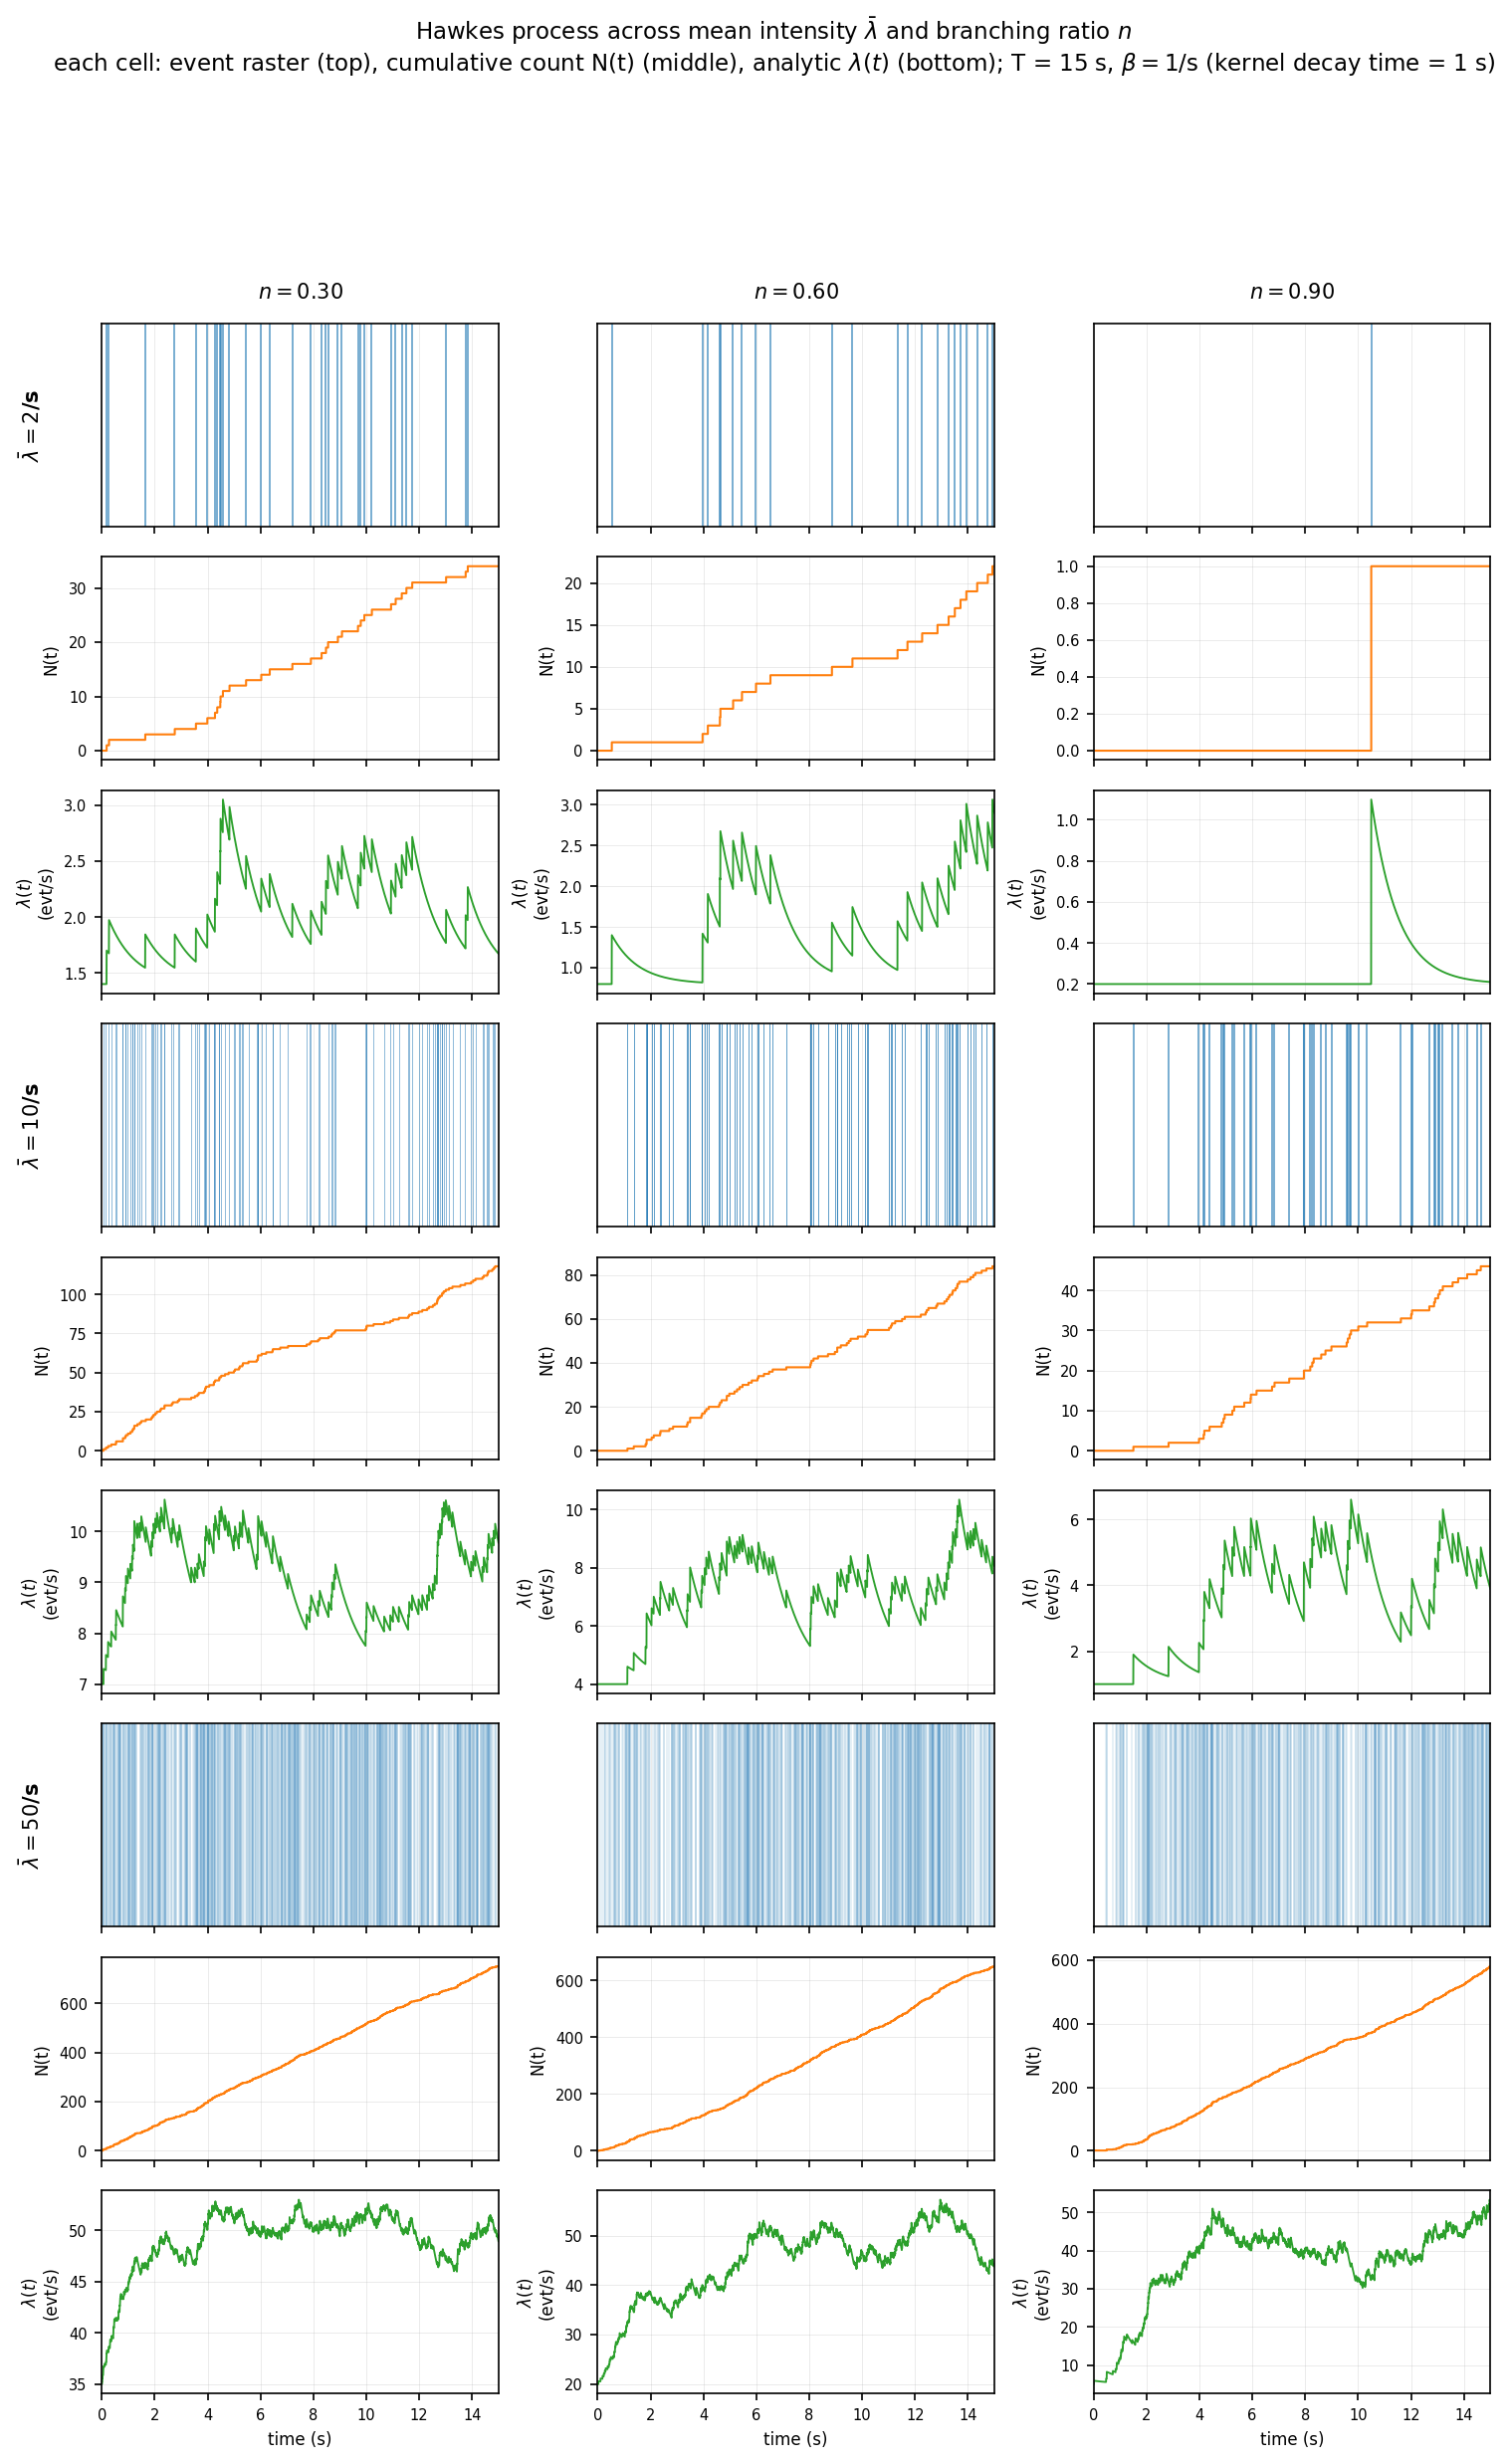
\includegraphics[width=\textwidth]{figs/hawkes_grid_3x3.png}
    \caption{Nine cells, each stacking the event raster (top), cumulative count $N(t)$ (middle), and analytic $\lambda(t)$ (bottom). Rows: mean intensity $\bar\lambda \in \{2, 10, 50\}$ events/s. Columns: branching ratio $n \in \{0.30, 0.60, 0.90\}$. Simulated by Ogata thinning over $15\,\mathrm{s}$ at $\beta = 1/$s. Generator: \texttt{arrival\_paper/make\_hawkes\_grid.py} (RNG seed pinned per cell for reproducibility).}
    \label{fig:hawkes-grid}
\end{figure}

\paragraph{The critical boundary.} At $n = 1$ exactly, the formula $\bar\lambda = \mu / (1 - n)$ diverges. On any finite window the process still fires finitely often, but the variance of $N(T)$ grows superlinearly with $T$. At $n > 1$ the process is supercritical and diverges in finite time; a well-behaved MLE on real data never returns $n > 1$ on a stable session. If a fit lands there it signals estimator instability, non-stationarity, or a mis-specified kernel. Our optimiser constrains $\alpha < \beta$ at the boundary and reports fits that hit the boundary as unreliable. Empirically, Filimonov--Sornette report $n \approx 0.85$--$0.95$ on ES over the 2000s--2010s; our own pilot on NQH5 2025-03-10 lands at $n = 0.90$, consistent with the near-critical-but-stable regime.

\subsection{Why Hawkes captures CME MDP3 and Poisson doesn't}
\label{app:pp-why-hawkes}

Three data signatures that a Poisson (or any renewal) process cannot produce, but Hawkes with $n$ close to 1 produces naturally:

\emph{(i) Very short interarrival gaps.} On ES/NQ book streams roughly 60--85\% of gaps are shorter than one-tenth of the mean gap. For any exponential the corresponding number is $1 - e^{-0.1} \approx 9.52\%$. Hawkes produces the excess of short gaps because each arrival transiently raises $\lambda$.

\emph{(ii) Positive gap autocorrelation.} For a Hawkes process $\mathrm{Corr}(\Delta_i, \Delta_{i+k}) > 0$ at every lag $k$. Long gaps cluster with long gaps (quiet periods), short with short (bursty periods). Renewal has i.i.d.\ gaps by definition, so the corresponding correlation is zero at every lag. Only self-excitation can produce positive lag-$k$ gap correlation.

\emph{(iii) Persistent burstiness across timescales.} The Fano factor $F(T)$ rises with the window size $T$ on a Hawkes process; on Poisson or any renewal it stays constant. Clustering isn't a single-timescale phenomenon --- it looks self-similar over decades of $T$.

\subsection{Fano factor: measuring dispersion of counts}
\label{app:pp-fano}

For a chosen window length $T$, chop the observation interval $[0, \tau_{\mathrm{end}}]$ into $K = \lfloor \tau_{\mathrm{end}}/T \rfloor$ disjoint bins. Let $C_k = N(kT) - N((k-1)T)$ be the count in bin $k$. The Fano factor at window $T$ is
$$F(T) = \frac{\mathrm{Var}[C_k]}{\mathrm{E}[C_k]}.$$
Poisson: $F(T) = 1$ for every $T$. This is the definitive Poisson signature. Hawkes / clustered: $F(T) > 1$, typically growing with $T$. Renewal: $F(T) \to 1$ as $T \to \infty$ because windows contain many i.i.d.\ gaps and the CLT kicks in. Rising Fano at large $T$ is therefore a Hawkes signature, not just a renewal signature. Origin: Fano (1947) in cosmic-ray physics.

\begin{figure}[H]
    \centering
    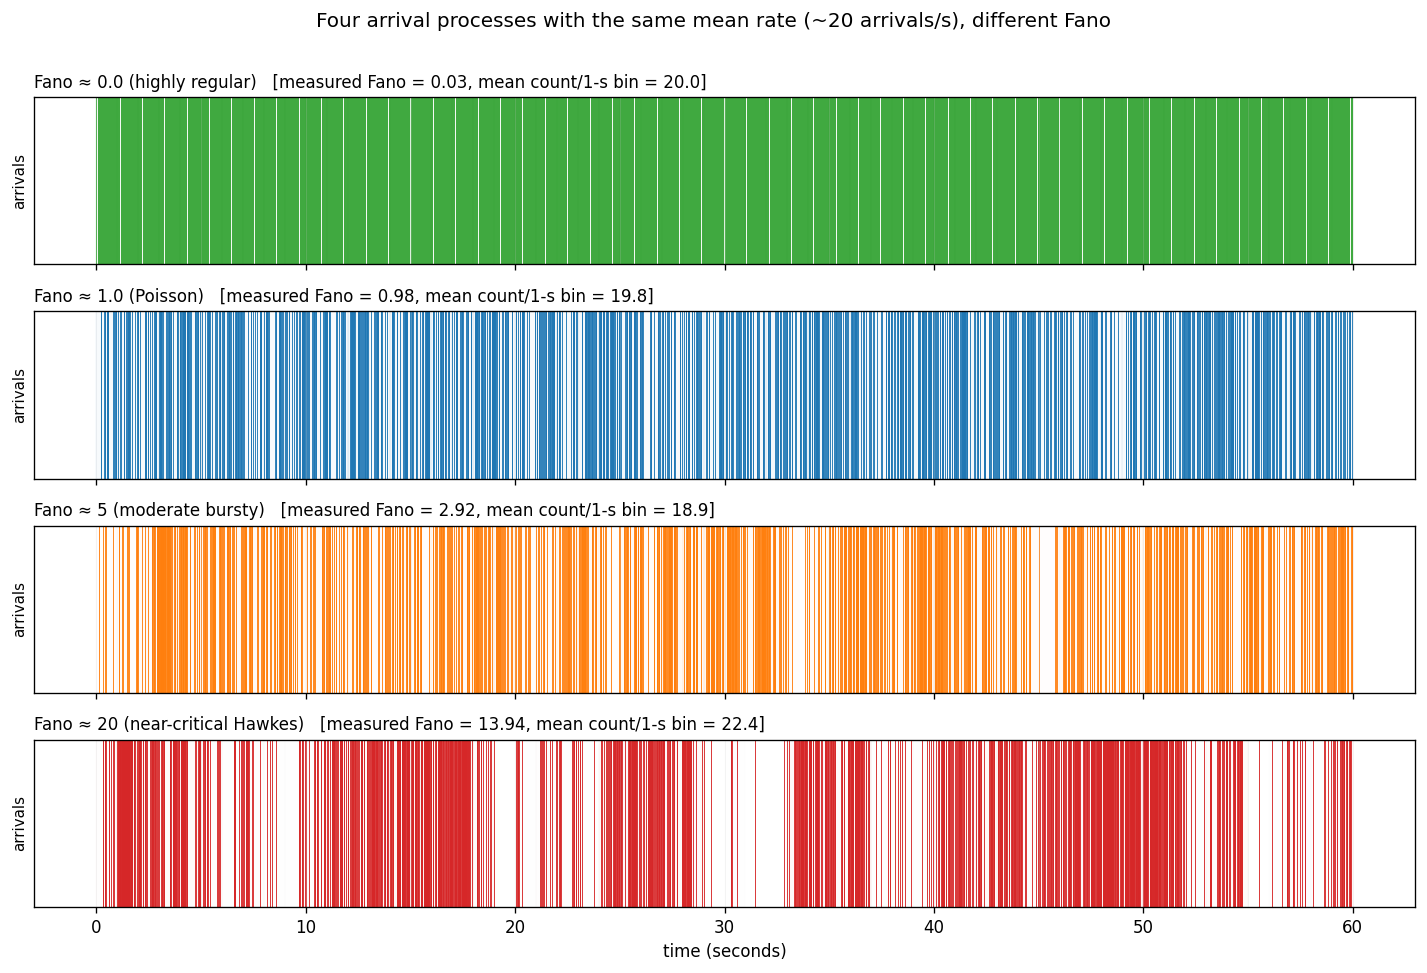
\includegraphics[width=\textwidth]{figs/rasters_by_fano.png}
    \caption{Same mean rate ($\sim 20$/s), four different processes. Top row ($F \approx 0$, highly regular): near-lattice cadence, bin counts nearly equal. Second row ($F \approx 1$, Poisson): the reference --- ``randomly spread'' with mildly uneven bin counts. Third row ($F \approx 3$, moderate Hawkes): visible clumping, bins 5--10 or 30--40. Bottom row ($F \approx 14$, near-critical Hawkes): pronounced bursts and long quiet stretches, bin counts from near zero to 50$+$.}
    \label{fig:rasters-fano}
\end{figure}

\begin{figure}[H]
    \centering
    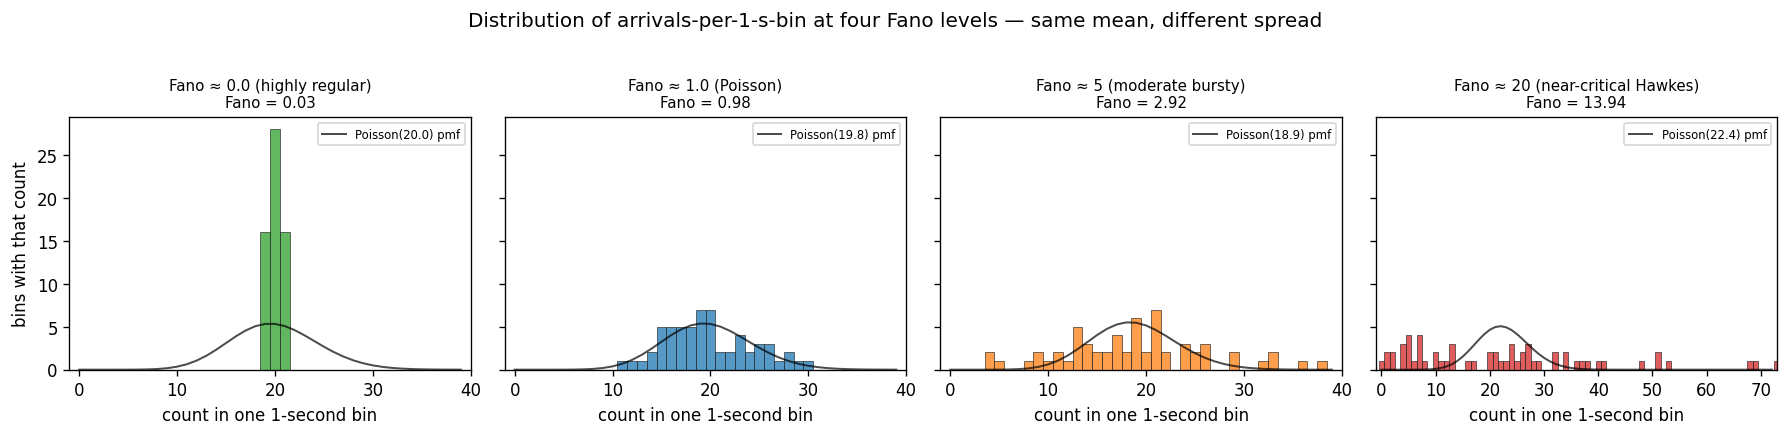
\includegraphics[width=\textwidth]{figs/count_hists_by_fano.png}
    \caption{Empirical distribution of arrivals per 1-second bin (bars) with Poisson pmf at same mean overlaid (curve). $F \approx 0$: histogram much narrower than Poisson --- sub-Poisson. $F \approx 1$: matches Poisson pmf. $F > 1$: wider than Poisson, extra mass in both tails --- what CME MDP3 looks like, shifted much further right ($F(1\,\mathrm{s})$ empirically 10--70 on ES/NQ MBO adds).}
    \label{fig:counthist-fano}
\end{figure}

\subsection{Hurst exponent: how burstiness scales with timescale}
\label{app:pp-hurst}

For a Hawkes-like process near criticality the Fano factor scales as a power law in the window size:
$$F(T) \sim T^{2H - 1},$$
where $H \in [0.5, 1)$ is the Hurst exponent. $H = 0.5$ means no long-range dependence (Poisson, renewal); $H > 0.5$ means long-range dependence, self-similar clustering across timescales; $H \to 1$ means extreme long memory. We estimate $H$ by OLS regression of log Fano on log window:
$$\log F(T) = (2H - 1)\log T + c + \varepsilon.$$
The fitted slope equals $2H - 1$, and $H = (\text{slope} + 1)/2$. For CME book feeds we typically observe $H \in [0.65, 0.75]$.

\begin{figure}[H]
    \centering
    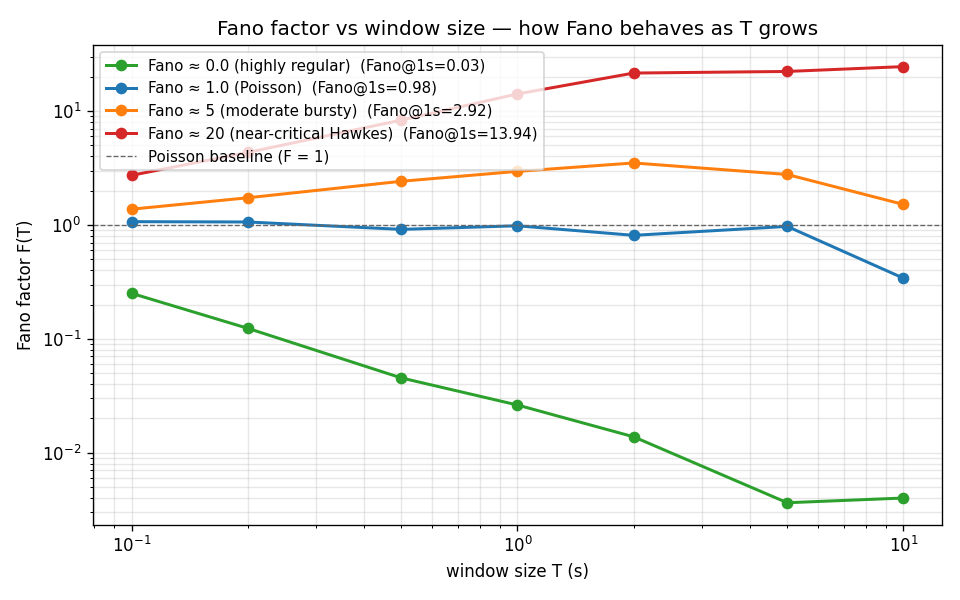
\includegraphics[width=0.75\textwidth]{figs/fano_scaling.png}
    \caption{Log-log $F(T)$ vs $T$ for four simulated processes. Regular: $F(T)$ near zero. Poisson: flat at $F = 1$. Moderate Hawkes: $F(T) > 1$ rising with $T$. Near-critical Hawkes: steep rise --- larger windows see bigger and bigger bursts. Slope of the log-log curve is $2H - 1$; the near-critical curve has slope $\approx 0.5$, corresponding to $H \approx 0.75$.}
    \label{fig:fano-scaling}
\end{figure}

Shuffling the gap sequence (Fisher--Yates permutation) preserves the marginal distribution of gaps exactly but destroys the ordering, thereby destroying any long-range dependence. Under shuffle $H_{\mathrm{shuffled}} \to 0.5$. This is our sharpest test for whether clustering lives in the ordering (Hawkes) or in the marginal (renewal).

\subsection{Notational summary}
\label{app:pp-notation}

\begin{center}
\begin{tabular}{@{}ll@{}}
\toprule
symbol & meaning \\
\midrule
$\Omega$ & sample space of all possible market days \\
$\mathcal{F}$ & $\sigma$-algebra of events \\
$\Pr(A)$ & probability of event $A \in \mathcal{F}$ \\
$\mathcal{F}_t$ & everything observable by time $t$ inclusive \\
$\mathcal{F}_{t^-}$ & everything observable strictly before $t$ \\
$t_1, t_2, \ldots$ & random arrival times \\
$N(t)$ & counting process: $\#\{i : t_i \leq t\}$ \\
$\lambda(t \mid \mathcal{F}_{t^-})$ & conditional intensity at $t$, units 1/time \\
$\mu$ & Hawkes background rate \\
$\phi(u)$ & Hawkes kernel \\
$\alpha$ & exp-kernel jump size \\
$\beta$ & exp-kernel decay rate (half-life $= \ln 2 / \beta$) \\
$\gamma$ & marked-Hawkes size exponent \\
$n = \int \phi$ & branching ratio; for exp kernel $n = \alpha/\beta$ \\
$\Delta_i = t_i - t_{i-1}$ & interarrival gap \\
$C_k$ & arrivals in bin $k$ under some window $T$ \\
$F(T)$ & Fano factor $= \mathrm{Var}[C_k] / \mathrm{E}[C_k]$ \\
$H$ & Hurst exponent, $F(T) \sim T^{2H-1}$ \\
$u_i$ & compensator increment $\int_{t_{i-1}}^{t_i} \lambda\, ds$ (\S\ref{app:pp-gof}) \\
\bottomrule
\end{tabular}
\end{center}

\section{Data --- what we compute from and where it lives}
\label{app:data}

\paragraph{Corpus.} CME MDP3 pre-decoded L3 record files (\texttt{.bin}) for ES (chan 310), NQ (chan 318), and BTC (chan 326, extraction in flight for 2025). Path: \texttt{/vast/home/vmayeski/out/bin/\{chan\}/\{chan\}.\{yyyymmdd\}.databento.bin}. Each record carries three ns-precision timestamps:

\begin{itemize}
    \item \texttt{transactTime} --- CME matching engine event time. The true arrival of the market event, stamped by CME's core matching engine and carried unchanged inside the MDP3 message body.
    \item \texttt{sendingTime} --- CME gateway UDP packet header time. Stamped by CME's outbound gateway when it packages matching-engine events into a UDP packet. The difference $\texttt{sendingTime} - \texttt{transactTime}$ measures CME-internal gateway queueing.
    \item \texttt{recv\_time} (on trades) / \texttt{handlerendtim} (on MBO records) --- the pcap wire-arrival timestamp at Databento's colo capture tap. Not our own capture: Databento captures pcaps in their CME-colo, stamps each UDP frame with the NIC-arrival time, and ships those pcaps to us. When we run \texttt{dbento\_pcap\_to\_bin}, \texttt{handler\_if.hpp} copies the pcap frame timestamp directly into the record's \texttt{handlerendtim} field on MBO messages and into \texttt{recv\_time} on trade messages (verified at \texttt{mdp3/include/mdp3/handler\_if.hpp:577,691,771,832} --- \texttt{l3.handlerendtim = recv\_time} unconditionally in the offline path). The field name \texttt{handlerendtim} is a misnomer inherited from the live-handler code path; in the historical corpus it functions as the pcap wire timestamp. The difference $\texttt{handlerendtim} - \texttt{sendingTime}$ measures CME-multicast transit to Databento's colo tap --- a network-only latency, cleanly separated from CME-internal queueing.
\end{itemize}

\paragraph{Important limitation.} The three-timestamp anatomy uses Databento's colo capture time, not our own. So the $\texttt{handlerendtim} - \texttt{sendingTime}$ distribution characterises the CME $\to$ Databento colo path, which is a stable colo-cross-connect path but is not literally the network we would see if we captured elsewhere. For arrival-process characterisation this does not matter --- the ordering and clustering of arrivals is invariant to any small fixed offset. For any latency-magnitude claim we call this out.

\paragraph{Field-name gotcha.} Older \texttt{handler\_if} code paths (live handlers) do write a genuine ``handler finished processing'' timestamp into \texttt{handlerendtim}. In the historical pcap pipeline we use, that same field is repurposed to carry the pcap wire timestamp.

\paragraph{Restrictions.} One front-month securityID per session (highest MBO Adds count in the day, from \texttt{binstats}). Roll days are dropped (front may straddle two contracts). RTH only, 09:30 $\to$ 16:00 ET. Overnight regime is future work. Message types: MBO records (\texttt{add}, \texttt{modify}, \texttt{cancel}, \texttt{execute}) plus MBO-trade records. Instrument-definition records (FDF/ODF/SDF) and volume/statistic records are excluded --- they are exchange bookkeeping, not order-flow arrivals.

\section{Model classes fit in this paper}
\label{app:models}

Three point-process models per (session, stream), in increasing complexity.

\subsection{Unmarked exponential Hawkes (the workhorse)}
\label{app:model-exp}

$$\lambda(t) = \mu + \sum_{t_i < t} \alpha\, e^{-\beta (t - t_i)}.$$
Three parameters: $\mu \geq 0$ (background), $\alpha \geq 0$ (jump), $\beta > 0$ (decay). Branching ratio $n = \alpha/\beta$. The exponential kernel is Markovian: intensity updates recursively in $O(1)$ per arrival, which is what makes the online estimator practical. Prior art (Hardiman--Bouchaud) warns the true kernel on CME data is closer to a power law; exponential is a working approximation over the timescales we care about ($100\,\mathrm{ms}$ --- $60\,\mathrm{s}$) and is the standard first step.

\subsection{Marked exponential Hawkes with size marks}
\label{app:model-marked}

$$\lambda(t) = \mu + \sum_{t_i < t} \alpha\,(1 + s_i)^\gamma\, e^{-\beta (t - t_i)}.$$
$s_i$ is a size mark: message size class (0--2 depending on quote or trade size deciles) or trade \texttt{lastQty}. $\gamma \geq 0$ measures how much larger events excite subsequent arrivals more than smaller events; LR test against the unmarked model verifies whether size marks meaningfully improve fit. Motivation: large trades and quote deletions plausibly carry more information than small ones.

\subsection{Bivariate Hawkes on \{bid-updates, ask-updates\}}
\label{app:model-bivariate}

Two intensities, one per side. Let $a, b \in \{\text{bid}, \text{ask}\}$:
$$\lambda_a(t) = \mu_a + \sum_{b} \sum_{t_i^{(b)} < t} \alpha_{ab}\, e^{-\beta_{ab}(t - t_i^{(b)})}.$$
$\alpha_{ab}$ is a $2 \times 2$ excitation matrix, diagonal terms $\alpha_{bb}, \alpha_{aa}$ = self-excitation, off-diagonal $\alpha_{ab}, \alpha_{ba}$ = cross-excitation. The $2 \times 2$ branching-ratio matrix has entries $K_{ab} = \alpha_{ab}/\beta_{ab}$; spectral radius of $K$ must be strictly less than 1 for stationarity. Cross-terms measure how much bid-side updates drag ask-side flow and vice versa --- the mechanical prediction that ``the book updates on both sides at once during price discovery.'' Underpins the directional signed-markout prediction in the main paper.

\section{Maximum-likelihood estimation}
\label{app:mle}

\subsection{What fitting a Hawkes actually means}
\label{app:mle-plain}

We have one input --- a sorted list of arrival times $t_1 < t_2 < \cdots < t_n$ for one session and one instrument --- and three knobs $(\mu, \alpha, \beta)$:

\begin{itemize}
    \item $\mu$ --- \textbf{exogenous rate}. Even if nothing has happened recently, events arrive at rate $\mu$ per second. Think ``rate at which news arrives''.
    \item $\alpha$ --- \textbf{jump size}. Every time an event happens, the intensity spikes up by $\alpha$. Units events/second. Think ``how much does one message beget others''.
    \item $\beta$ --- \textbf{decay rate}. Each spike from $\alpha$ fades exponentially with time constant $1/\beta$. Units 1/second. Think ``how fast does excitement fade''.
\end{itemize}

Fitting means: turn the three knobs until the model gives the observed timestamps the highest probability. Formally, maximise the log-likelihood \eqref{eq:hawkes-loglik}. Intuitively, if $\alpha$ is too low the model can't explain visible burst-clustering; if $\alpha$ is too high (approaching $\beta$) the model over-predicts explosive clustering; if $\mu$ is too high or too low the model mis-explains quiet periods. The optimiser tries settings until it finds the triple $(\hat\mu, \hat\alpha, \hat\beta)$ that maximises the log-likelihood.

Once we have the fit, we measure: (i) intensity $\lambda(t)$ --- plug $(\hat\mu, \hat\alpha, \hat\beta)$ into the formula to get $\lambda(t)$ at any $t$, high when arrivals have been clustering, low when the market has been quiet; (ii) branching ratio $n = \alpha/\beta$; (iii) long-run mean intensity $\bar\lambda = \mu/(1 - n)$ --- the stationary expected arrival rate, $\mu$ amplified by $1/(1 - n)$ through self-excitation.

\paragraph{Numerical example (NQH5, 2025-03-10).} On the pilot session:
$$\hat\mu = 0.45\ \text{events/s}, \qquad \hat\alpha = 0.068, \qquad \hat\beta = 0.076,$$
giving branching ratio $\hat n = 0.68/0.076 \approx 0.90$ and long-run mean intensity $\bar\lambda \approx 4.5$ events/s. NQ was strongly self-exciting on that session (near-critical), the exogenous news rate was small (0.45/s), and the observed mean rate of $\sim 5/$s was carried mostly by cascading self-excitation rather than fresh news.

\subsection{Log-likelihood}
\label{app:mle-loglik}

Write $\theta$ for the parameter vector ($(\mu, \alpha, \beta)$ for the unmarked model, $(\mu, \alpha, \beta, \gamma)$ for marked, etc.) and $\log L(\theta)$ for the log-likelihood. For a point process with intensity $\lambda(\cdot; \theta)$ observed on $[0, T]$ with events $t_1, \ldots, t_n$, the log-likelihood is standard \citep{ozaki1979}:
\begin{equation}
\log L(\theta) = \sum_{i=1}^n \log \lambda(t_i; \theta) - \int_0^T \lambda(s; \theta)\, ds.
\label{eq:hawkes-loglik}
\end{equation}
The first term rewards high intensity at the times events actually happened; the second (subtracted) term penalises models that predict too many events overall.

For the exponential Hawkes both terms have closed-form $O(n)$ recursions. Introduce
$$R_i = e^{-\beta(t_i - t_{i-1})}(1 + R_{i-1}), \qquad R_0 \equiv 0,$$
so $\lambda(t_i) = \mu + \alpha R_i$ and
$$\sum_{i=1}^n \log \lambda(t_i) = \sum_{i=1}^n \log(\mu + \alpha R_i).$$
The compensator has the closed form
$$\int_0^T \lambda(s)\, ds = \mu T + \frac{\alpha}{\beta}\sum_{i=1}^n\!\big(1 - e^{-\beta(T - t_i)}\big).$$
Marked and bivariate generalisations are analogous.

\subsection{Optimiser}
\label{app:mle-opt}

Python \texttt{scipy.optimize.minimize} with L-BFGS-B (Limited-memory Broyden--Fletcher--Goldfarb--Shanno with box constraints), a quasi-Newton optimiser that climbs the log-likelihood using local gradient information without the full Hessian and enforces our parameter bounds. Analytic gradient supplied. Bounds: $\mu \geq 0$, $\alpha \geq 0$, $\beta > 0$, and for marked $\gamma \geq 0$. Warm-start from method-of-moments initial estimates. Fit time per RTH session on the 72-core box: seconds for the unmarked model, tens of seconds for marked, minutes for bivariate.

\subsection{Numerical stability}
\label{app:mle-stab}

Sub-second precision timestamps must be shifted to a session-relative origin $t_i \leftarrow t_i - t_0$ before optimisation; otherwise the $\exp(-\beta t_i)$ terms underflow for wall-clock ns timestamps. On very active sessions ($n > 10^7$) we sub-sample uniformly to $n \approx 10^6$ for the fit, then verify on the full sequence. Uniform sub-sampling is not stationary-Hawkes-preserving in the strict sense but produces stable parameter estimates in practice.

\section{Diagnostic statistics --- the per-session panel row}
\label{app:diag}

Everything above sets up the vocabulary and the models. This section says: \emph{for one trading session on one stream, this is exactly what we compute}. Run it $731$ days $\times$ $3$ streams (ES/NQ/BTC) and you get the $\sim 2200$-row panel that every downstream result in the paper reads from.

\paragraph{One session, one stream $\to$ one row of the panel.} Each session on each stream produces roughly 25--30 scalars that fit on a single row. The row is written to disk as JSON at \texttt{/vast/home/vmayeski/out/arrival\_paper/fits/\{stream\}/\{yyyymmdd\}.hawkes.json}; the $\sim 2200$ daily rows are concatenated into \texttt{/vast/home/vmayeski/out/arrival\_paper/panels/hawkes\_panel.parquet}. That panel is the paper's empirical evidence base.

\paragraph{Two kinds of statistics: model-free and model-dependent.} Model-free stats (\S\ref{app:diag-marginal}--\S\ref{app:diag-order}) come first as a sanity check --- any point-process reader can reproduce them without fitting anything. Fit-dependent stats (\S\ref{app:diag-nrec}--\S\ref{app:pp-gof}) tell us whether the Hawkes we fit actually explains the data.

\begin{center}
\begin{tabular}{@{}llll@{}}
\toprule
subsection & what it computes & type & scalars \\
\midrule
\S\ref{app:diag-marginal} Marginal-gap stats & CV, quantile ratios, $\Pr(\text{gap}<\text{mean}/10)$ & model-free & $\sim 10$ \\
\S\ref{app:diag-fano} Fano scaling + Hurst & $F(T)$ at 5 windows, $H$ from slope & model-free & $\sim 6$ \\
\S\ref{app:diag-order} Gap ACF + shuffle test & ACF at 5 lags, shuffled $F(5\,\mathrm{s})$, collapse & model-free & $\sim 7$ \\
\S\ref{app:diag-nrec} Branching-ratio recovery & $n$ MLE, $n$ MoM, gap & fit-dependent & $\sim 3$ \\
\S\ref{app:pp-gof} Goodness-of-fit & KS $p$, Ljung-Box $p_{20}$, QQ plot & fit-dependent & $\sim 2$ \\
\bottomrule
\end{tabular}
\end{center}

Baseline expectations under a homogeneous Poisson at the same mean rate are given in parentheses throughout. Departures from those baselines are the paper's evidence.

\subsection{Marginal-gap statistics}
\label{app:diag-marginal}

\begin{itemize}
    \item \textbf{Coefficient of variation:} $\mathrm{CV} = \sigma(\Delta)/\mathrm{E}[\Delta]$ (Poisson: 1.0).
    \item \textbf{Squared CV:} $\mathrm{CV}^2$ (Poisson: 1.0).
    \item \textbf{Quantile ratios:} p10, p50, p90, p99, p99.9 gaps against $\mathrm{Exp}(\text{same mean})$ quantiles $-m \log(1 - p)$. Ratio crosses 1 exactly once for a burst process.
    \item $\Pr(\text{gap} < \text{mean}/10)$: 9.52\% for any exponential; empirically 40--85\% on CME book streams.
    \item \textbf{Instantaneous rate:} mean rate vs rate implied by median gap. $1/\log 2 \approx 1.44 \times$ for any exponential; empirically 14--120$\times$ on CME.
\end{itemize}

\subsection{Count-based statistics --- Fano scaling and Hurst}
\label{app:diag-fano}

Windowed count in the $k$-th bin: $N_T(k) = N(kT) - N((k-1)T)$. Fano at window $T$: $F(T) = \mathrm{Var}[N_T]/\mathrm{E}[N_T]$ (Poisson: 1 at every $T$). Compute $F(T)$ at $T \in \{0.1, 1, 5, 60, 300\}$ seconds. Fit the log-log regression by OLS to extract the Hurst exponent:
$$\log F(T) \approx (2H - 1)\log T + c.$$
$H = 0.5$ Poisson or renewal, $H \in (0.5, 1)$ long-range dependence characteristic of Hawkes, $H > 1$ non-stationary or diverging variance.

\subsection{Ordering statistics --- gap ACF and shuffle test}
\label{app:diag-order}

Renewal processes with heavy-tailed marginals can produce large CV and moderate Fano without any ordering-driven clustering. To separate the two:

\begin{itemize}
    \item \textbf{Gap ACF} at lags 1, 2, 3, 5, 10. Positive at all lags means long-gap-follows-long-gap.
    \item \textbf{Fisher--Yates shuffle:} seeded permutation of the gap sequence preserves the marginal exactly and destroys the ordering. Recompute $F(5\,\mathrm{s})$ and $H$ on the shuffled sequence. The collapse ratio
    $$\text{collapse} = \frac{F_{\text{original}}(5\,\mathrm{s})}{F_{\text{shuffled}}(5\,\mathrm{s})}$$
    measures how much clustering lives in the ordering versus the marginal. Near 1 = renewal; much greater than 1 (empirically 3--19$\times$ on ES/NQ book streams) = Hawkes. The shuffle is the definitive test: renewal is invariant under shuffle, Hawkes is not.
\end{itemize}

\subsection{Branching-ratio recovery}
\label{app:diag-nrec}

For fitted Hawkes, $n = \alpha/\beta$ directly from the fit. Sanity check against the method-of-moments estimator, which is model-free and uses only the Fano ceiling:
$$n_{\mathrm{MoM}} \leq 1 - \frac{1}{\sqrt{F(T \to \infty)}}.$$
Discrepancy larger than 10\% is a red flag for either misspecification (wrong kernel family) or non-stationarity within the session.

\subsection{Goodness-of-fit --- time-rescaling}
\label{app:pp-gof}

The time-rescaling theorem is a classical result: if we knew the true intensity $\lambda(\cdot)$, integrating it between consecutive events gives compensator increments
$$u_i = \int_{t_{i-1}}^{t_i} \lambda(s)\, ds$$
that are i.i.d.\ $\mathrm{Exp}(1)$ under the correct model. In practice we transform back to uniform via $p_i = 1 - e^{-u_i}$, which should be i.i.d.\ $U(0, 1)$ under the correct model. We then apply:

\begin{itemize}
    \item \textbf{Kolmogorov--Smirnov test} against $U(0, 1)$. Compares the empirical CDF to the target CDF; the statistic is the maximum absolute gap. Small $p$ means the model does not fit. Report $p_{\mathrm{KS}}$ per session.
    \item \textbf{Ljung--Box test} on the $u_i$ for serial correlation --- a joint test that the first several autocorrelations are zero. Small $p$ flags remaining autocorrelation. Report $p_{\mathrm{LB}}$ at lag 20.
    \item \textbf{QQ plot} on $\mathrm{Exp}(1)$ --- plot each residual's rank against its expected $\mathrm{Exp}(1)$ quantile; points fall on $y = x$ if the model fits. Visual, one representative session per stream in the paper.
\end{itemize}

Empirical target: $p_{\mathrm{KS}} > 0.05$ on $\geq 80\%$ of sessions. Failure at this rate on a given stream would indicate the exponential kernel is too restrictive and we would move to a power-law kernel (Hardiman--Bouchaud), a mixture of exponentials, or a marked model.
